\section{Introduction}
\label{sec:intro}


I had always been fascinated with mathematical shapes and curves. One day, I stumbled onto a toy called the Spirograph. Although I never owned a set at home, I admired the beautiful drawings that it produced. As a little project, I was inspired to write a computer program that could simulate a Spirograph. In order to do that, I needed to first understand how a Spirograph moved. \\

The mathematics behind spirographs 

We have a circle centered on the origin with radius $R$. Let's draw a line from the origin to the radius at an angle $\alpha$ counter-clockwise from the origin. 

\begin{figure}[h]
    \centering
    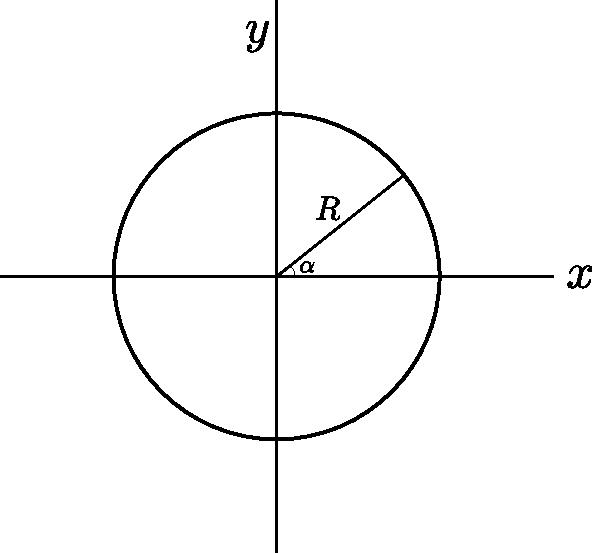
\includegraphics[width=8cm]{figures/unitcircle1.pdf}    
    \caption{Caption}
    \label{fig:my_label}
\end{figure}
This creates a right-angled triangle with hypotenuse a hypotenuse (R) and vertical and horizontal legs which are opposite and adjacent to angle $\alpha$. By definition, \\
\begin{center}
$sin(\alpha) = \frac{Opp}{Hyp} = \frac{Opp}{R} \Rightarrow Rsin(\alpha) = Opp $
\\
$cos(\alpha) = \frac{Adj}{Hyp} = \frac{Adj}{R} \Rightarrow Rcos(\alpha) = Adj $
\end{center}

\begin{figure}[H]
    \centering
    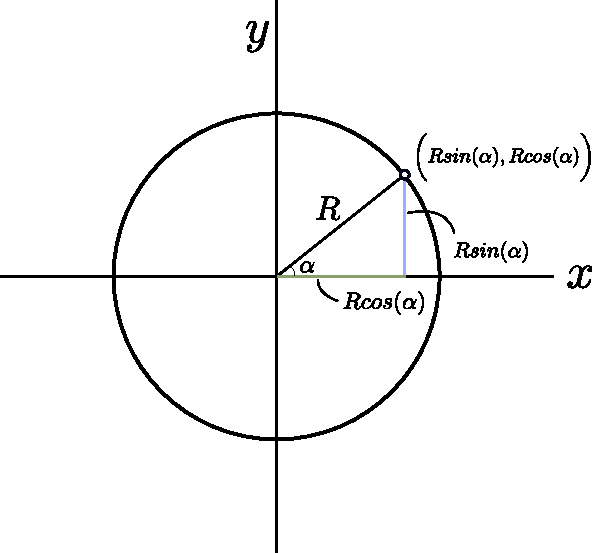
\includegraphics[width=8cm]{figures/unitcircle2.pdf}    
    \caption{Caption}
    \label{fig:my_label}
\end{figure}

We are interested in describing the epicycloid. To do this, we must add in another circle on the surface of the original circle.

\begin{figure}[H]
    \centering
    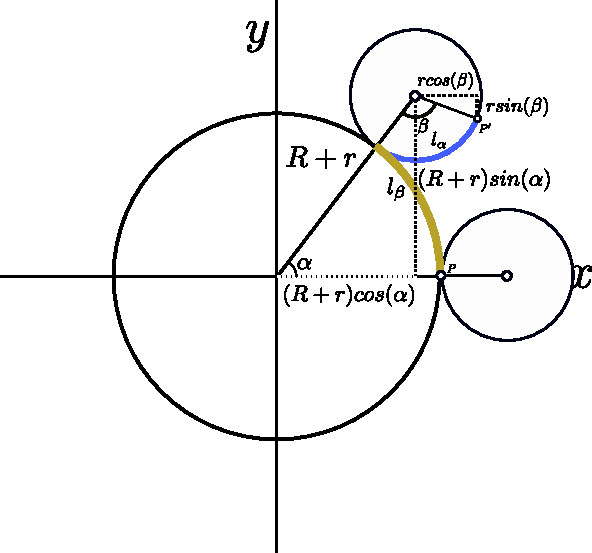
\includegraphics[width=8cm]{figures/epicycloid1.pdf}    
    \caption{Caption}
    \label{fig:my_label}
\end{figure}

For convention, we fix the "pen" at the point at the point of contact between the small and large circle, and the small circle is placed directly to the right of the large circle. At some moment after beginning to roll, the small circle be located at an angle $\alpha$ from the $x$-axis. The "pen" will have rotated at an angle $\beta$ relative to the small circle, and an angle $\alpha+\beta$ relative to the center of the large circle. 

In this configuration, the parametric equations for the epicycloid will be
\begin{centering}

$y = (R+r)sin(\alpha) - rsin(\alpha+\beta)$ \\ 
$x = (R+r)cos(\alpha) - rcos(\alpha+\beta)$ \\ 

\end{centering}
The 




We can express $\beta$ in terms of $\alpha$ with one key insight: The small circle rolls on the surface of the large circle. This means that the arc length travelled on the large circle is the same as the arc length travelled on the small circle. We can express the following:

\begin{centering}
$l_\alpha = l_\beta$ \\
\end{centering}

Arc length is defined to be a portion of the total circumference of the circle given by an angle and a full rotation. In radians, this is: \\

\begin{centering}
$l = 2\pi r(\dfrac{\theta}{2\pi}) = r\theta $ \\
\end{centering} 

Applying this to our arc lengths $l_\alpha$ and $l_\beta$: \\
\begin{centering}
$ R\alpha = r\beta$ \\
$\dfrac{R}{r}\alpha = \beta$ \\
\end{centering} 


We can substitute this into our equations to obtain the parametric equations of a epicycloid:

\begin{centering}
$y(\alpha) = (R+r)sin(\alpha) - rsin(\frac{R+r}{r}\alpha)$ \\ 
$x(\alpha) = (R+r)cos(\alpha) - rcos(\frac{R+r}{r}\alpha)$ \\ 
\end{centering}

Since an epicycloid involves \textit{rolling motion} and \textit{motion} involves \textit{time}, I substituted $\alpha$ with $t$ (representing time). This is just for conventional purposes.

\begin{centering}
$y(t) = (R+r)sin(t) - rsin(\frac{R+r}{r}t)$ \\ 
$x(t) = (R+r)cos(t) - rcos(\frac{R+r}{r}t)$ \\ 
\end{centering}

Now that the equations of the epicycloid are derived, I wrote them into a computer program and generated various figures, with $R$ and $r$ as constants and $t$ as a variable. 


The equations of the epicycle can be parameterized into the complex plane using using Euler's identity:

\begin{centering}
$e^{ix} = isin(\theta) + cos(\theta)$
\end{centering}

Notice in our original parametric equations that there are two sets of sines and cosines - one set of sine and cosine representing the y and x coordinates large circle, and another set representing y and x coordinates of the small circle.


To the ancients, the defining feature of the planets was that they ``wander'' or undergo retrograde motion. Mathematically, we can determine when exactly a planet undergoes retrograde motion by taking the derivative of its parametric equations. When its velocity is negative, it can be assumed that the planet is undergoing retrograde motion.

For any general deferent and single epicycle system with general equations

$y = y(t) = r_{0}sin(v_{0}t) + r_{1}sin(v_{1}t)$ \\
$x = x(t) = r_{0}cos(v_{0}t) + r_{1}cos(v_{1}t)$ \\ 

The derivative will be 
$ \frac{dy}{dx} = \frac{y'(t)}{x'(t)}$ \\
$ y'(t) = r_{0}v_{0}cos(v_{0}t) $



\begin{centering}
$z(\alpha) = (R+r)e^{i\alpha}-re^{\frac{r+R}{r}i\alpha}$
\end{centering}